\let\negmedspace\undefined
\let\negthickspace\undefined
\documentclass[journal]{article}
\usepackage[a5paper, margin=10mm, onecolumn]{geometry}
\usepackage{lmodern} % Ensure lmodern is loaded for pdflatex

\setlength{\headheight}{1cm} % Set the height of the header box
\setlength{\headsep}{0mm}     % Set the distance between the header box and the top of the text

\usepackage{gvv-book}
\usepackage{gvv}
\usepackage{cite}
\usepackage{textcomp}
\usepackage{amsmath,amssymb,amsfonts,amsthm}
\usepackage{algorithmic}
\usepackage{graphicx}
\graphicspath{{./figs/}}
\usepackage{textcomp}
\usepackage{xcolor}
\usepackage{txfonts}
\usepackage{listings}
\usepackage{enumitem}
\usepackage{mathtools}
\usepackage{gensymb}
\usepackage{comment}
\usepackage[breaklinks=true]{hyperref}
\usepackage{tkz-euclide} 
\usepackage{listings}
\usepackage{gvv}                                        
\def\inputGnumericTable{}                                 
\usepackage[latin1]{inputenc}                                
\usepackage{color}                                            
\usepackage{array}                                            
\usepackage{longtable}                                       
\usepackage{calc}                                             
\usepackage{multirow}                                         
\usepackage{hhline}                                           
\usepackage{ifthen}                                           
\usepackage{lscape}
\usepackage{circuitikz}
\tikzstyle{block} = [rectangle, draw, fill=blue!20, 
text width=4em, text centered, rounded corners, minimum height=3em]
\tikzstyle{sum} = [draw, fill=blue!10, circle, minimum size=1cm, node distance=1.5cm]
\tikzstyle{input} = [coordinate]
\tikzstyle{output} = [coordinate]


\begin{document}
	
	\bibliographystyle{IEEEtran}
	\vspace{3cm}
	
\title{4.7.44}
\author{EE25BTECH11047 - RAVULA SHASHANK REDDY}
\maketitle
\hrulefill
\bigskip 

\renewcommand{\thetable}{\theenumi}
\setlength{\intextsep}{10pt}

\textbf{Question:}  \\

Find the distance of the plane from the origin.
\begin{align*}
\vec{r}^T\myvec{\tfrac{2}{7}\\[4pt]\tfrac{3}{7}\\[4pt]-\tfrac{6}{7}} = 1
\end{align*}

\textbf{Solution:} \\ 

Equation of plane
\begin{align}
    \vec{n}^T \vec{x} &= 1,\\
    \vec{n} &= \myvec{\tfrac{2}{7}\\[4pt]\tfrac{3}{7}\\[4pt]-\tfrac{6}{7}}.\\
    d &= \frac{|\vec{n}^T \vec{x}_0 - 1|}{\|\vec{n}\|}.\\
    d &= \frac{|\vec{n}^T \vec{0} - 1|}{\|\vec{n}\|} \\
      &= \frac{|0 - 1|}{\|\vec{n}\|} \\
      &= \frac{1}{\|\vec{n}\|}.\\
    \|\vec{n}\| &= \sqrt{\vec{n}^T \vec{n}} \\
    &= \sqrt{\left(\tfrac{2}{7}\right)^2 + \left(\tfrac{3}{7}\right)^2 + \left(-\tfrac{6}{7}\right)^2} \\
    &= \sqrt{\tfrac{49}{49}} \\
    &= 1.
\end{align}

Therefore, the required distance is
\begin{align}
    d &= \frac{1}{1} = \boxed{1}.
\end{align}
\newpage
\begin{figure}
    \centering
    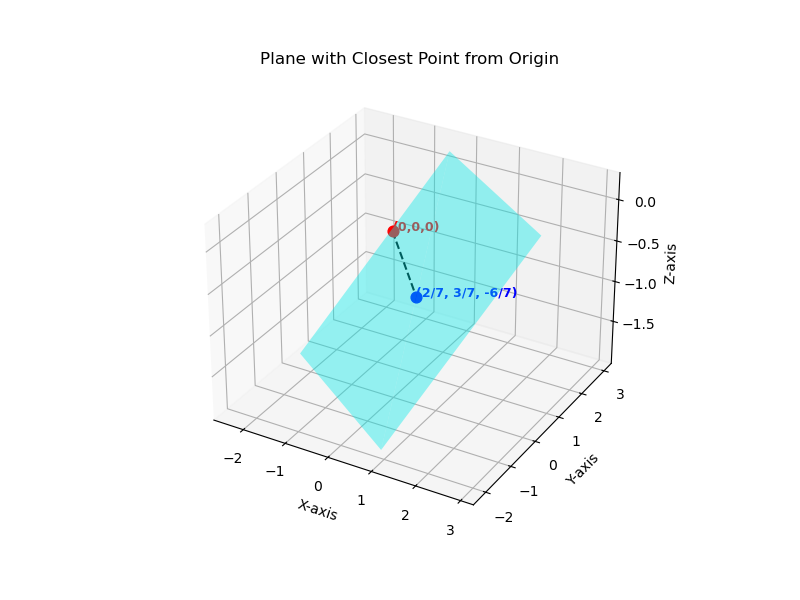
\includegraphics[width=1.0\linewidth]{figs/fig1.png}
    \caption{}
    \label{fig:placeholder}
\end{figure}
\end{document}

